\section{\textsc{Salatsauce mit Joghurt}}

\subsection*{Zutaten für 300ml:}

\begin{tabular}{p{7.5cm} p{7.5cm}}
	& \\
	250g Joghurt & 10ml Orangensaft \\
	10ml Öl & 5ml Zitronensaft \\
	Worcestersauce & Salz \& Pfeffer
\end{tabular}

\subsection*{Serviervorschlag:}

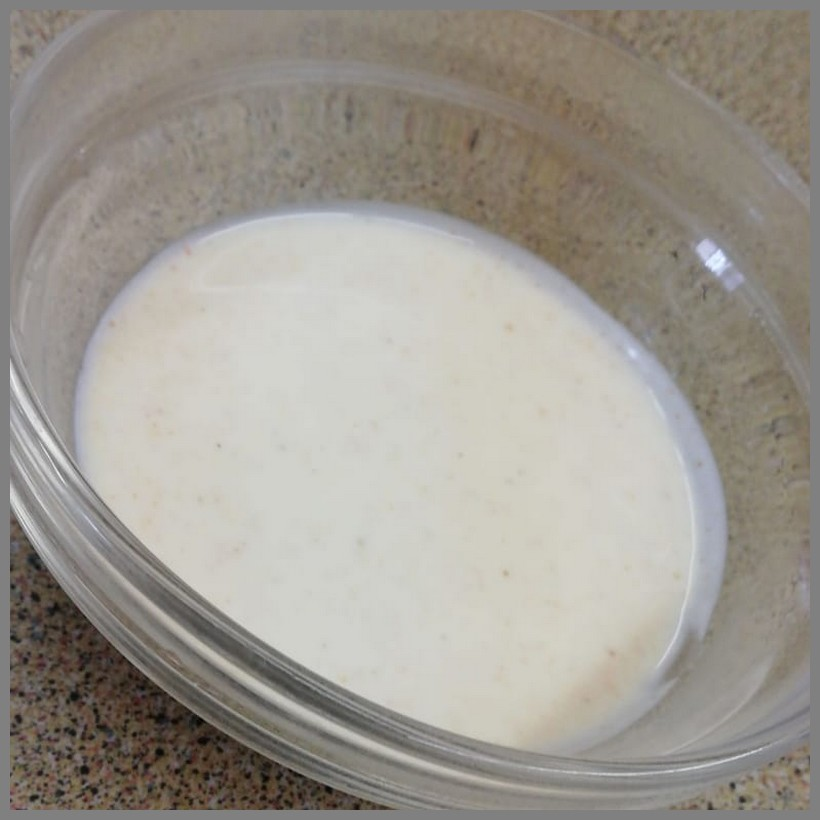
\includegraphics[width=\textwidth]{img/d_joghurt.jpeg} \cite{djoghurt}

\subsection*{So geht's:}

\begin{tabular}{p{15cm}}
	\\
	Joghurt, Orangen- und Zitronensaft mit einem Spritzer Worcestersauce zu einer glatten Masse verühren.\\
	Öl unterrühren und mit Salz und Pfeffer abschmecken.\\
	\\
	Geeignet zu allen Salaten.
\end{tabular}
